\documentclass[12pt,a4paper]{report}
\usepackage[utf8]{inputenc}
\usepackage[francais]{babel}
\usepackage[T1]{fontenc}
\usepackage{amsmath}
\usepackage{amsfonts}
\usepackage{amssymb}
\usepackage{url}
\usepackage{ucs}
\usepackage{graphicx}
\usepackage{lmodern}
\usepackage{xcolor}
\usepackage[left=2cm,right=2cm,top=2cm,bottom=2cm]{geometry}
\author{Typhaine PL}
\setcounter{tocdepth}{1} 
\usepackage{lmodern}
\usepackage{fancyvrb}
\definecolor{Zgris}{rgb}{0.87,0.85,0.85}

% Pour avoir du code coloré
\usepackage{listings}
\lstset{
language=HTML,        % choix du langage
basicstyle=\ttfamily\footnotesize,       % taille de la police du code
keywordstyle=\ttfamily\bfseries\color{red},  %style des mots clefs
commentstyle=\ttfamily\slshape\color{darkgreen},  %style des commentaires
identifierstyle=  \ttfamily\color{blue},  %style des identificateurs
stringstyle= \ttfamily\color{green},  %style des chaines de caractères
showstringspaces=false,
numbers=left,                   % placer les numéros de lignes à gauche (left)
numberstyle=\footnotesize,        % taille de la police des numéros
numbersep=6pt,            % distance entre le code et sa numérotation
tabsize=4,
xleftmargin=17pt,
escapeinside={\%*}{*)},
breaklines=true,
breakatwhitespace=true,
string=[b]{'}
}

\newsavebox{\BBbox}
\newenvironment{DDbox}[1]{
\begin{lrbox}{\BBbox}\begin{minipage}{\linewidth}}
{\end{minipage}\end{lrbox}\noindent\colorbox{Zgris}{\usebox{\BBbox}} \\
[.5cm]}

\makeatletter
\def\clap#1{\hbox to 0pt{\hss #1\hss}}%
\def\ligne#1{%
\hbox to \hsize{%
\vbox{\centering #1}}}%
\def\haut#1#2#3{%
\hbox to \hsize{%
\rlap{\vtop{\raggedright #1}}%
\hss
\clap{\vtop{\centering #2}}%
\hss
\llap{\vtop{\raggedleft #3}}}}%
\def\bas#1#2#3{%
\hbox to \hsize{%
\rlap{\vbox{\raggedright #1}}%
\hss
\clap{\vbox{\centering #2}}%
\hss
\llap{\vbox{\raggedleft #3}}}}%
\def\maketitle{%
\thispagestyle{empty}\vbox to \vsize{%
\haut{}{\@blurb}{}
\vfill
\vspace{1cm}
\begin{flushleft}
\usefont{OT1}{ptm}{m}{n}
\huge \@title
\end{flushleft}
\par
\hrule height 4pt
\par
\begin{flushright}
\usefont{OT1}{phv}{m}{n}
\Large \@author
\par
\end{flushright}
\vspace{1cm}
\vfill
\begin{center}
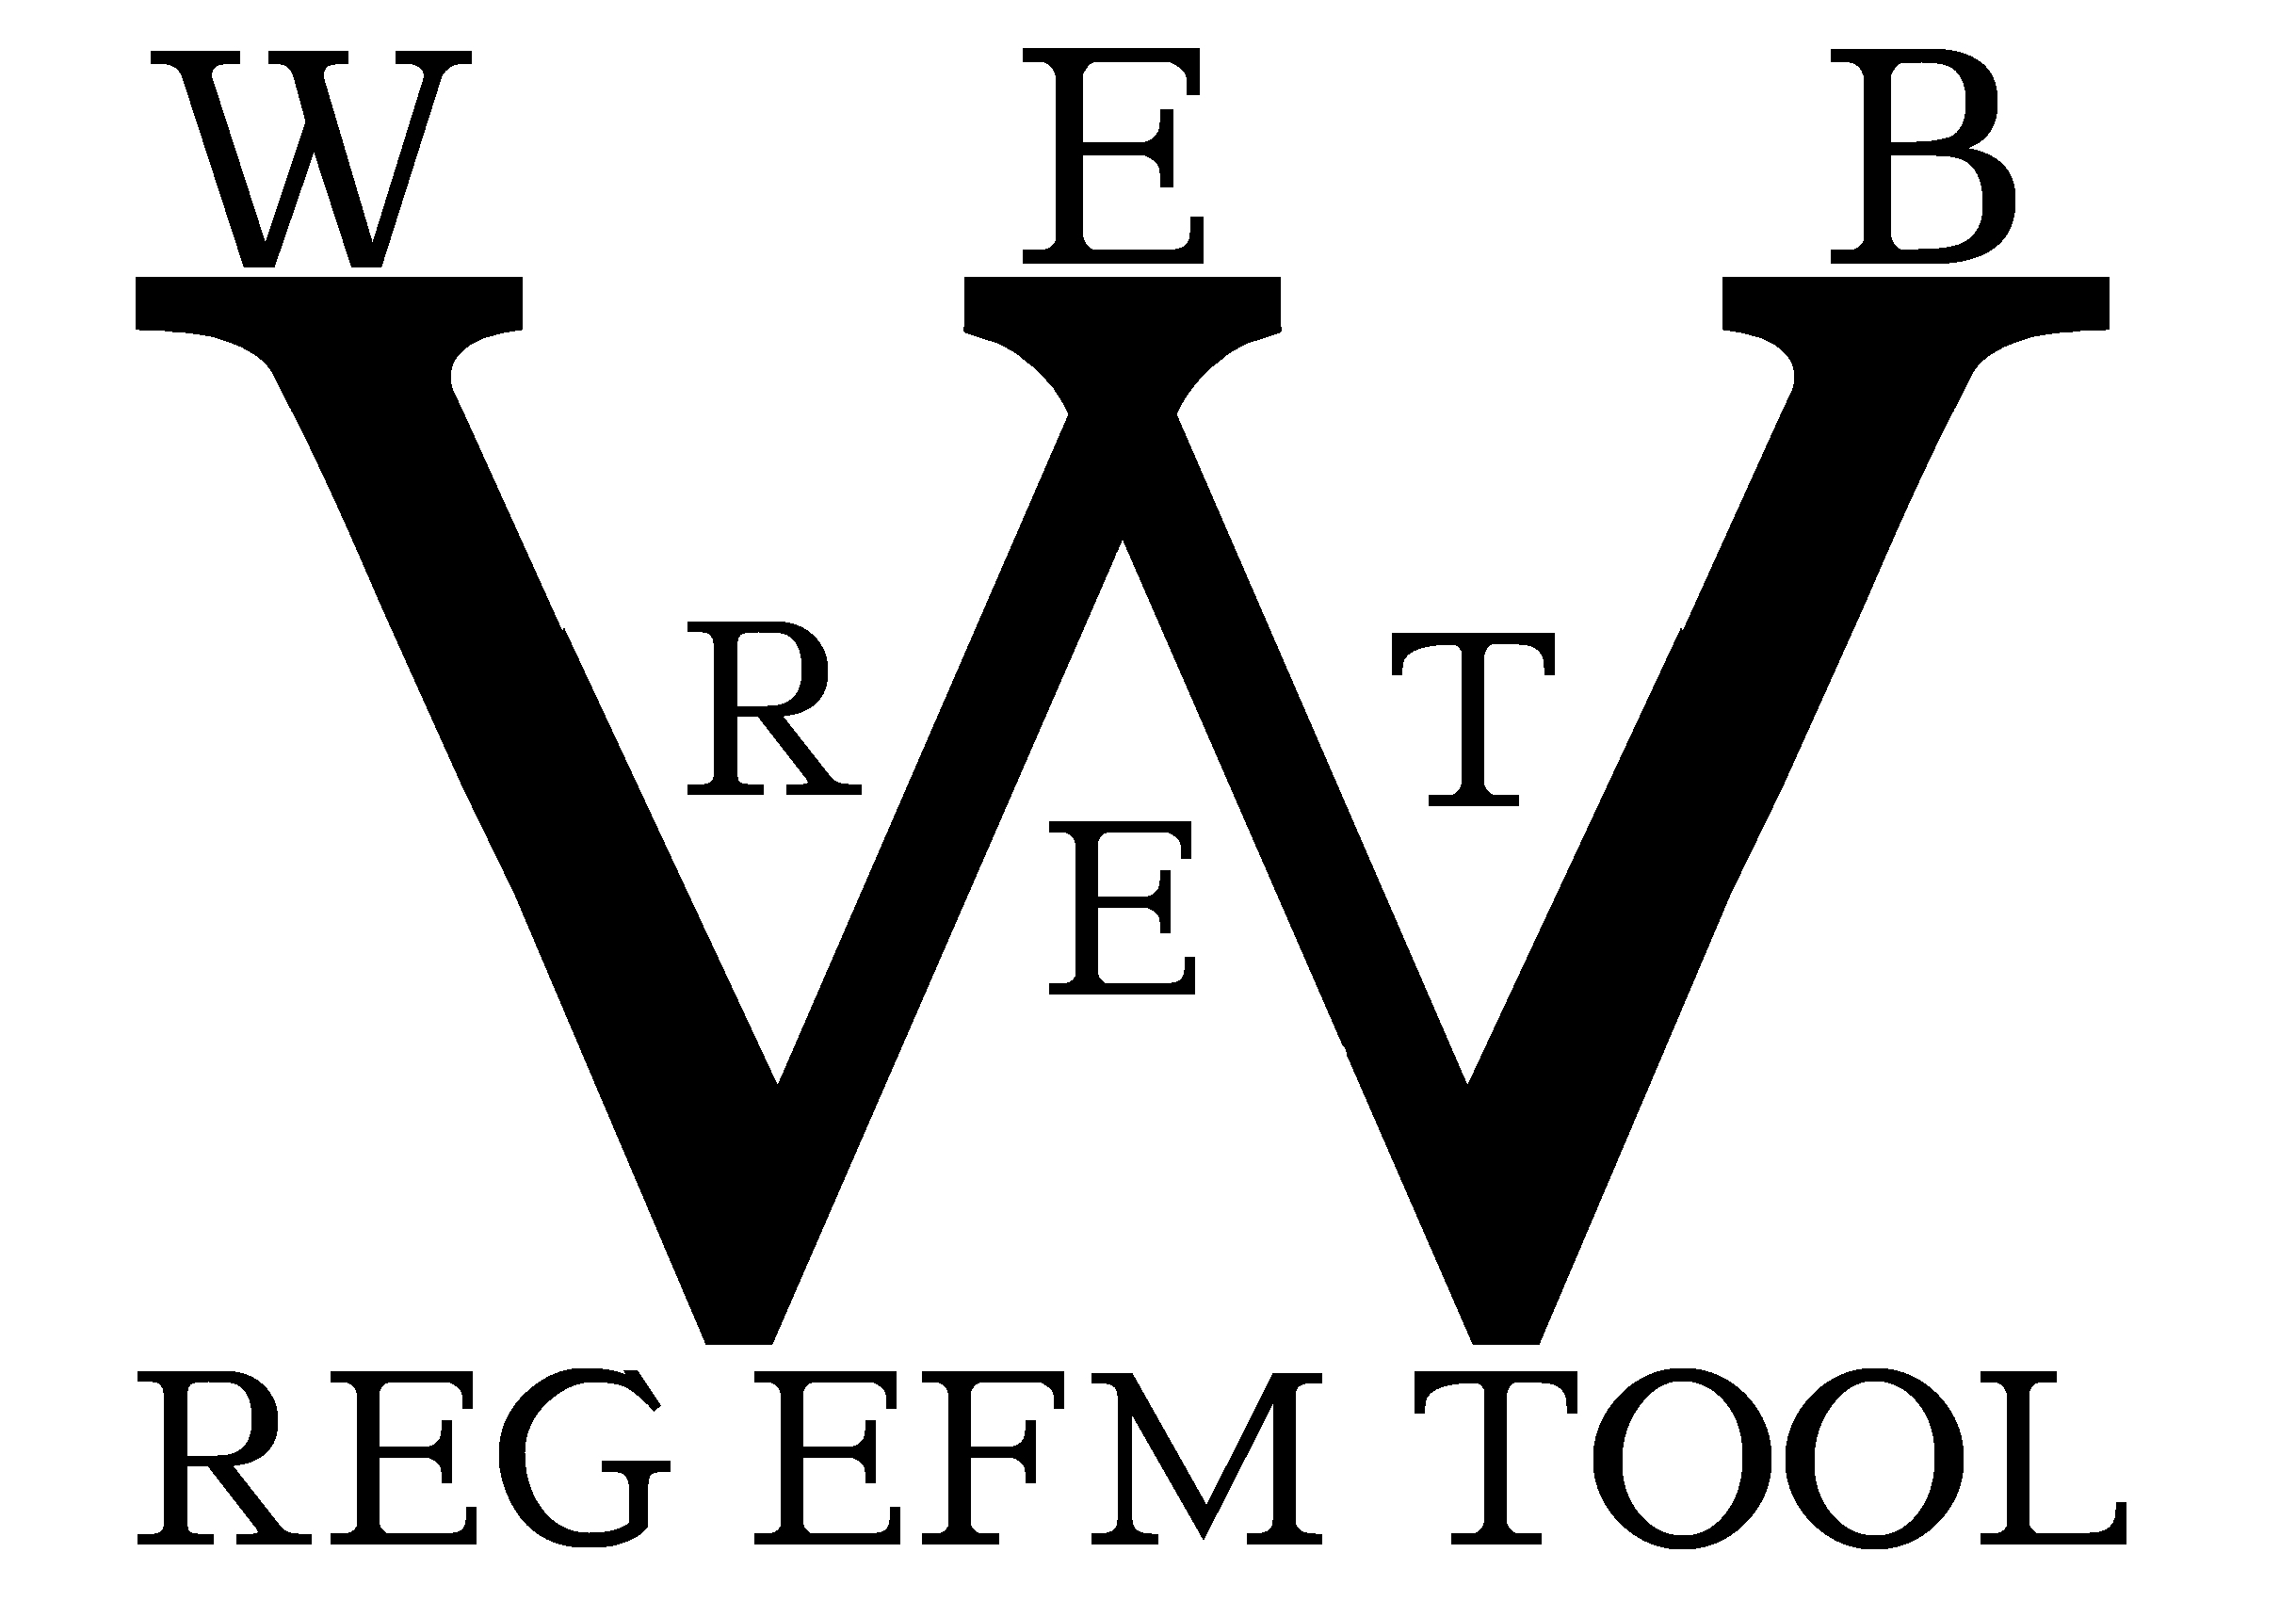
\includegraphics[width=0.3\textwidth]{../Images/logo/logo.png}\\
\vspace{2cm}

\includegraphics[width=0.1\textwidth]{../Images/logounibdx.png}
\end{center}
\vfill
\bas{}{\@date}{}
}%
\cleardoublepage
}
\def\date#1{\def\@date{#1}}
\def\author#1{\def\@author{#1}}
\def\title#1{\def\@title{#1}}
\def\location#1{\def\@location{#1}}
\def\blurb#1{\def\@blurb{#1}}
\date{\today}
\author{}
\title{}
\location{}\blurb{}
\makeatother

\title{Manuel d'installation}
\author{\textsc{FR\`ECHE} Arnaud, \textsc{H\'ERIC\'E} Charlotte, \textsc{MOLA} Saraï,\\ \textsc{PAYSAN-LAFOSSE} Typhaine, \textsc{SANSEN} Joris}
\location{Bordeaux}
\blurb{%
Universités de Bordeaux\\
Master 2 BioInformatique
\textbf{}\\[1em]
\textsc{Marie \textsc{Beurton-Aimar}}
}%

\begin{document}
\maketitle
\tableofcontents


\chapter{WRET}
\section{Pré-requis}
WRET est une interface pour le logiciel \textit{regEfmtool} 2.0. Ce dernier doit \^etre installé pour le bon fonctionnement de la page Web.

Ce manuel a pour but de préciser les installations à effectuer pour WRET.

\section{Définition}

Cette interface nommée \emph{WRET : WebRegEfmTool} permet de générer les fichiers nécessaires à l'utilisation du logiciel de modélisation \textit{regEfmtool}. Elle permet également la création de réseaux au format \emph{DAT} afin de lancer des simulations comparées sur le logiciel METATOOL.

\section{Téléchargement d'Apache}

Apache est un serveur web HTTP (Hypertext Transfer Protocol) et permet de construire des sites Web dynamiques. Il est autonome, très complet et permet ainsi de fournir la manutention de sessions automatiques (avec ou sans cookies), la gestion des erreurs et un accès facile aux paramètres GET et POST envoyées par le client.

Le téléchargement de Apache se trouve sur la page \url{http://www.apachefriends.org/en/xampp-linux.html}. Le paquet ainsi que les étapes d'installation s'y trouvent.


\section{Installation}

Tout d'abord, la version correspondant au système d'exploitation de la machine doit être téléchargé. Par la suite les commandes suivantes sont à entrer dans un terminal:\\
\texttt{\$ su\\
\$ tar xvfz xampp-linux-1.8.1.tar.gz -C /opt\\}

Pour lancer serveur Apache, il suffit simplement d'entrer la commande \texttt{\$ /opt/lampp/lampp start} dans un terminal.
\chapter{RegEfmtool}

\textit{RegEfmtool} fonctionne avec le langage de programmation Java. Java 1.7 est la version minimale qui permet de faire fonctionner ce logiciel.

\section{Définition}

Le logiciel \textit{regEfmtool} permet la modélisation de réseaux métaboliques et le calcul de modes élémentaires. Ce logiciel fonctionne sous environnement \emph{UNIX} uniquement en ligne de commandes et nécessite plusieurs fichiers d'entrée au format texte. Ces derniers doivent être générés à la main et contiennent les informations sur ce réseau. Sa prise en main n'est donc pas aisée pour un utilisateur ne possédant aucune connaissance en programmation.\\


\section{Téléchargement}

Le téléchargement de \textit{regEfmtool} se fait depuis la page \url{http://www.biotec.boku.ac.at/regulatoryelementaryfluxmode.html} . La version 2.0 s'y trouve ainsi que de nombreuses informations sur son installation, ses dépendances, sa licence et des contacts.

\section{Installation}

Java doit être installé préalablement sur la machine. Prenons l'exemple de XAMPP : se placer dans le dossier /opt/lamp/htdocs/xampp de votre machine. Le paquet 20120810\_regEfmtool\_2.0.tar.gz doit y est installé. \\
Dans une fenêtre de terminal, les commandes suivantes sont à entrer:\\
\texttt{\$tar -xvfz 20120810\_regEfmtool\_2.0.tar.gz\\
\$ which javac\\
\$ which jar\\}

Ouvrir le Makefile pour modifier le chemin absolu de JAR et JAVAC. Puis finir avec les commande suivante dans le Terminal:\\
\texttt{\$ make\\
\$ make jarfile\\}

Pour vérifier si le logiciel est bien installé réaliser les commandes suivantes dans un terminal :\\
\texttt{\$ cd examples
\$ ./start\_regEfmtool\_simple\_1}

Si tout est bien installé, les résultats de la commande devraient s'afficher dans le Terminal.

\end{document}